\documentclass[12pt]{book}
\usepackage[dvipsnames]{xcolor}
\usepackage{amssymb,latexsym}
\usepackage{graphicx}

\usepackage[spanish,mexico,es-nolayout]{babel}
\usepackage[utf8]{inputenc}
\usepackage{amsmath}
\DeclareMathOperator{\tr}{tr}
% \usepackage{amssymb}
\usepackage{amsthm}
%\usepackage{graphicx}
\usepackage{color}
\usepackage{tikz}
\usepackage{tkz-berge}
\usepackage{makeidx}
\usepackage{url}
\usepackage{xspace}
\usepackage{tocbibind}
% ver http://gilmation.com/articles/latex-margins-for-book-binding/
% y http://tex.stackexchange.com/questions/50258/margins-of-book-class
\usepackage[margin=3.5cm]{geometry}
\geometry{bindingoffset=1cm}

%\usepackage{babelbib}

\usetikzlibrary{positioning,shapes,fit,arrows,decorations.pathmorphing}
\definecolor{myblue}{RGB}{56,94,141}


\newtheorem{theorem}{Teorema}[section]
\newtheorem{corollary}[theorem]{Corolario}
\newtheorem{proposition}[theorem]{Proposición}

\theoremstyle{definition}

\newtheorem{definition}[theorem]{Definición}
\newtheorem{notation}[theorem]{Notación}
\newtheorem{example}[theorem]{Ejemplo}
\newtheorem{lemma}[theorem]{Lema}

\newcounter{in}
\newcounter{ini}

\DeclareMathOperator{\Cay}{Cay}
\DeclareMathOperator{\diam}{diam}
\DeclareMathOperator{\Stab}{Stab}
\DeclareMathOperator{\Aut}{Aut}
\DeclareMathOperator{\orb}{Orb}

\newcommand{\GAP}{\textsf{GAP}\xspace}
\newcommand{\GRAPE}{\textsf{GRAPE}\xspace}

\makeindex

\newcommand{\elespacio}{1.4cm}

\begin{document}
\mainmatter 
\begin{titlepage}
  \begin{center}
    \null
    \vspace*{\fill}

    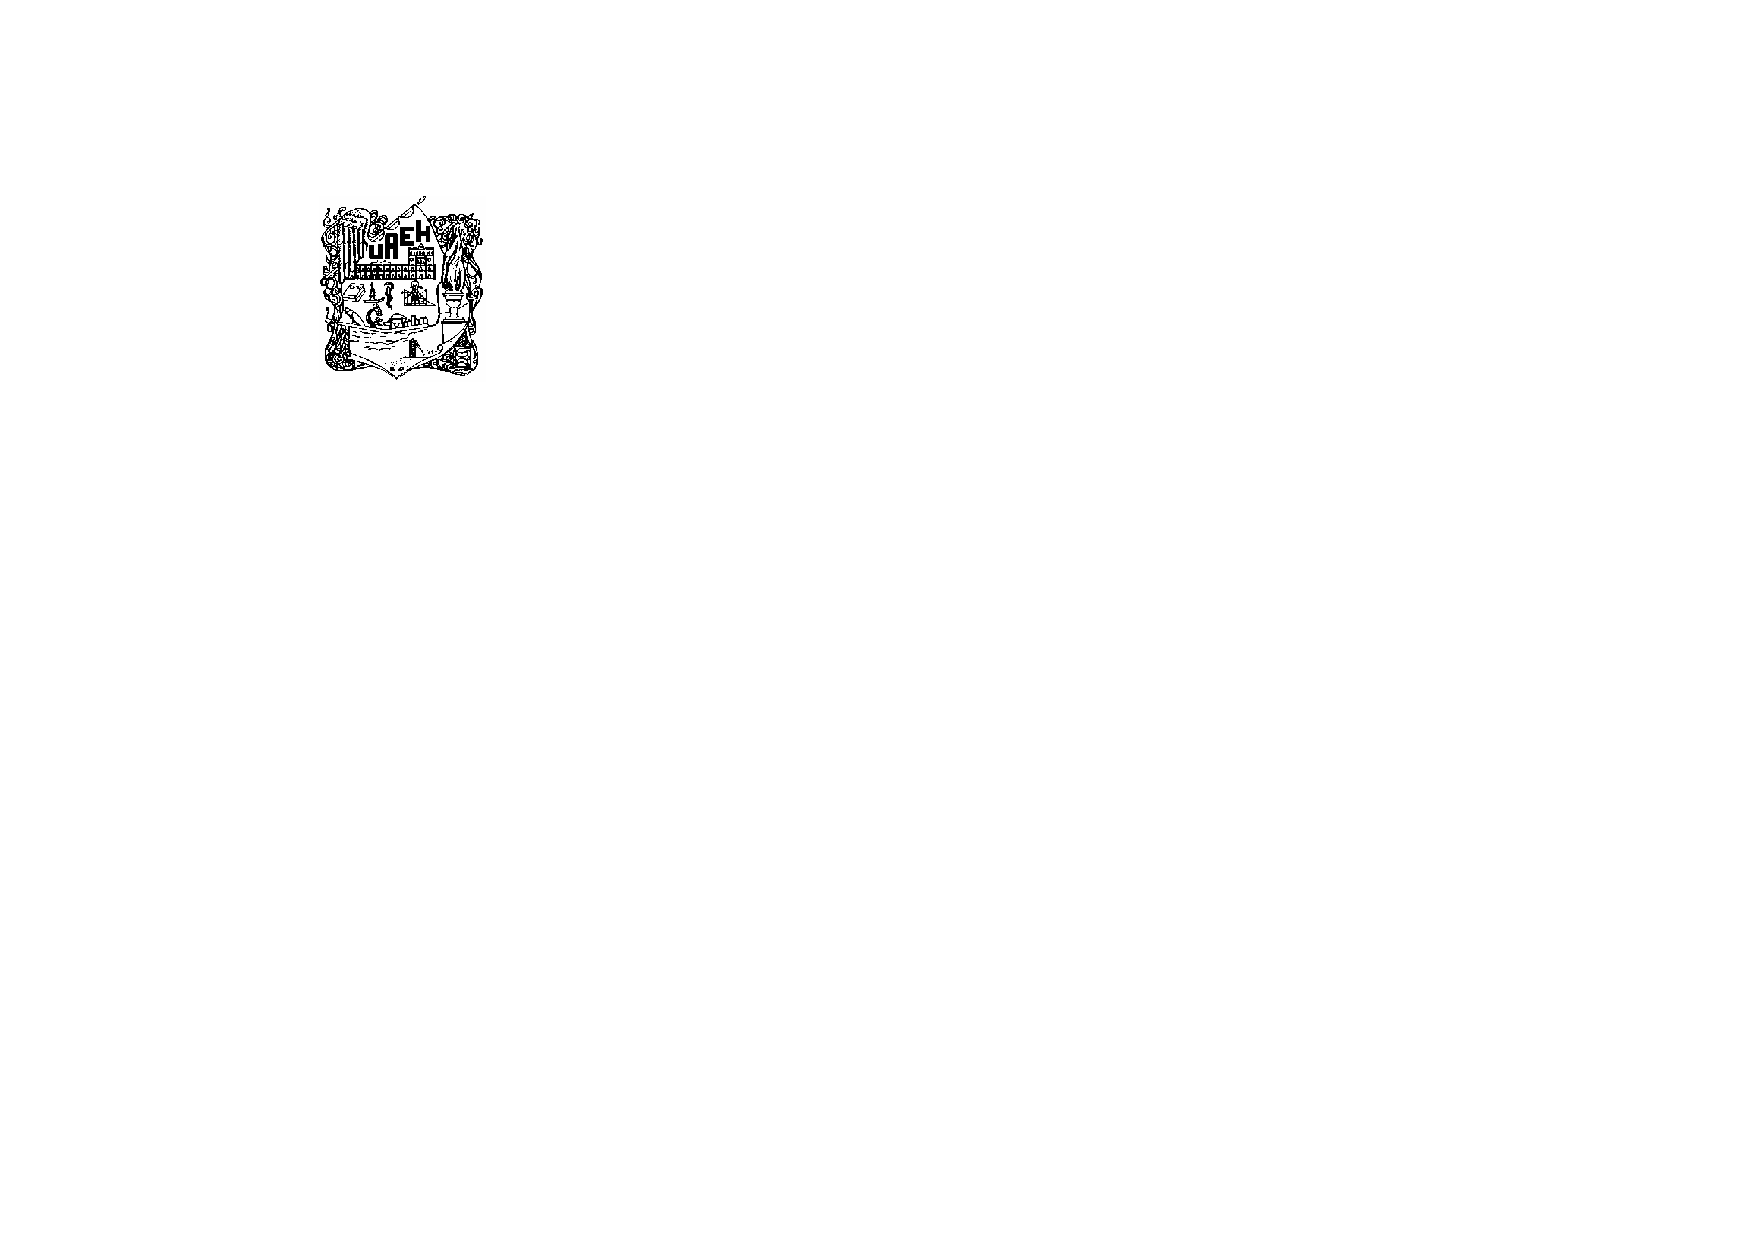
\includegraphics[scale=1.2,bb=55 20 0 0]{escudouaeh.pdf}

    \vspace*{\elespacio}

    \textsc{Universidad Autónoma del Estado de Hidalgo}

    \textsc{Instituto de Ciencias Básicas e Ingeniería}

    \textsc{Área Académica de Matemáticas y Física}

    \vspace*{\elespacio}

    {\Huge\bfseries Un enfoque computacional de representaciones de
      grupos en homologías\par}

    \vspace*{\elespacio}

    {\large Tesis que para obtener el título de}

    \vspace*{\elespacio}

    {\Large\textsc{Licenciado en Matemáticas Aplicadas}}

    \vspace*{\elespacio}

    {\large presenta}

    \vspace*{\elespacio}

    {\Huge Manuel Campero Jurado}

    \vspace*{\elespacio}

    {\large bajo la dirección de}

    \bigskip

    {\Large Dr.~Rafael Villarroel Flores}

    \bigskip

    {Pachuca, Hidalgo. Octubre de 2018.}

    \vspace*{\fill}

  \end{center}
\end{titlepage}

\thispagestyle{empty}
\begin{flushleft}
  {\bfseries\Large Resumen}
\end{flushleft}

En esta tesis se hace blah blah blah blah blah blah blah blah blah
blah blah blah blah blah blah blah blah blah.

\vspace{2cm}

\begin{flushleft}
  {\bfseries\Large Abstract}
\end{flushleft}

In this thesis blah blah blah blah blah blah blah blah blah
blah blah blah blah blah blah blah blah blah.

 \newpage \thispagestyle{empty}

\chapter{Representaciones de grupos}
\label{cha:Representaciones de grupos}

En este capítulo veremos las definiciones básicas de representaciones
de grupos. La presentación está basada en \cite{MR882540}.

\section{Definiciones básicas}
\label{sec:basicas}

Sea $ \mathrm{GL}(n,\mathbb{C})$ el grupo de todas las matrices no
singulares $n\times n$ sobre el campo de los números complejos
$\mathbb{C}$. Sea $G$ un grupo. Una representación (matricial) de $G$
se define como un homomorfismo:
\begin{equation*}
  A \colon a \mapsto \mathrm{GL}(n,\mathbb{C})
\end{equation*}
el cual por definición cumple
\begin{enumerate}
\item $A\left(ab\right)=A\left(a\right)A\left(b\right)$,
\item $A\left(1\right)=I_{n}$ (la matriz identidad $n\times n$),
\item $A\left(a^{-1}\right)=A\left(a\right)^{-1}$.
\end{enumerate}
El número $n$ se llama el grado de la representación. Se dice que la
representación es fiel si $A$ es inyectiva.

\begin{example}
  \label{Ej6}
  La función que manda cada elemento de $G$ a $1
  \in \mathbb{C}$ es una representación de grado 1. Ésta es llamada la
  representación unitaria de $G$, y es denotada por $1_{G}$. 
\end{example}
 
\begin{example}
  \label{Ej5}
  Dadas una representación $A$ y una matriz no singular $P$, la regla:
  \begin{equation*}
    a \mapsto P^{-1}A\left(a\right)P
  \end{equation*}  
  induce una representación de $G$.

  Sean $A$ y $B$ representaciones de $G$. Si existe una
  matriz no singular $P$ tal que para todo $a \in G$:
  \begin{equation*}
    B\left(a\right)= P^{-1}A\left(a\right)P
  \end{equation*}
  entonces se dirá que $A$ y $B$ son equivalentes. Representaciones
  equivalentes se denotan como $A \sim B$. La relación $\sim$ define
  una clase de equivalencia de representaciones de $G$.
\end{example}

\begin{example}
  \label{Ej3}
  Sea $S_{n}$ el grupo simétrico de grado
  $n$. Para un elemento
  \begin{equation}
    \label{eq:1}
    \sigma =
    \begin{pmatrix}
      1 & 2 & \cdots  & n\\
      s_{1} & s_{2} & \cdots & s_{n}
    \end{pmatrix} 
    \in S_{n},
  \end{equation}
  y sea
  \begin{equation*}
    \alpha_{ij}\left(\sigma\right) = \left\{
      \begin{array}{ll}
        1      & \mathrm{si\ } j = s_{i} \\
        0      & \mathrm{otro\ caso\ }, 
      \end{array}
    \right.
  \end{equation*}
  entonces definimos $A\left(\sigma\right)$ como la matriz cuyo
  $i$-ésimo renglón es $\left(0,...,0,1,0,...,0\right)$ con 1 en el
  $s_{i}$-ésimo lugar, por lo cual para $\left(i,j=1,2,...,n\right)$
  se tiene:
  \begin{equation*}
    A\left(\sigma\right) = \left(\alpha_{ij}\left(\sigma\right)\right).
  \end{equation*}
  La regla $\sigma \mapsto A\left(\sigma\right)$ es una representación
  fiel de $S_{n}$.
\end{example}


\begin{example}
  \label{Ej4}
  Sea $G$ un grupo finito cuyos elementos son $a_{1},a_{2},...,a_{n}$
  y sea $S^{G}$ el grupo simétrico en $G$. La función bajo la cual
  cada elemento $a \in G$ es llevado a la permutación \ref{eq:6} es un
  homomorfismo inyectivo de $G$ en $S^{G}$.
  \begin{equation}
    \label{eq:6}
    \begin{pmatrix}
      a_{1} & a_{2} & \cdots  & a_{n}\\
      a_{1}a & a_{2}a & \cdots & a_{n}a
    \end{pmatrix} 
    \in S_{n}^{G}.
  \end{equation}
  Sea
  \begin{equation*}
    \alpha_{ij} (a) = \left\{
      \begin{array}{ll}
        1      & \mathrm{si\ } a_{i}a = a_{j} \\
        0      & \mathrm{otro\ caso\ }, 
      \end{array}
    \right. 
  \end{equation*}
  entonces a \ref{eq:6} se le asocia la matriz. 
  \begin{equation*}
    A(a)=\big(\alpha_{ij}(a)\big).
  \end{equation*} 
  Entonces la regla $a \mapsto A\left(\sigma\right)$ se convierte en
  una representación fiel de $G$. A ésta se le llama representación
  regular derecha de $G$. Es decir, que para $\delta{(a)}$ como 
  \begin{equation*}
    \delta{(a)} = \left\{
      \begin{array}{ll}
        1      & \mathrm{si\ } a = 1 \\
        0      & \mathrm{otro\ caso,\ } 
      \end{array}
    \right.
  \end{equation*}
  entonces se tiene la siguiente matriz, y se observa que si
  $a \neq 1$ cada elemento sobre la diagonal es cero.
  \begin{equation}
    \label{eq:7}
    A\left(a\right) = 
    \begin{pmatrix}
      \delta\left(a_{1}aa_{1}^{-1}\right) & \delta\left(a_{1}aa_{2}^{-1}\right) & \cdots  & \delta\left(a_{1}aa_{n}^{-1}\right)\\
      \delta\left(a_{2}aa_{1}^{-1}\right) & \delta\left(a_{2}aa_{2}^{-1}\right) & \cdots  & \delta\left(a_{2}aa_{n}^{-1}\right)\\ 
      \vdots & \vdots & \ddots & \vdots\\
      \delta\left(a_{n}aa_{1}^{-1}\right) & \delta\left(a_{n}aa_{2}^{-1}\right) & \cdots  & \delta\left(a_{n}aa_{n}^{-1}\right)
    \end{pmatrix}
    .
  \end{equation}

  La representación regular izquierda de $G$ se define análogamente
  usando el siguiente homomorfismo:
  \begin{equation*}
    a \mapsto
    \begin{pmatrix}
      a_{1} & a_{2} & \cdots  & a_{n}\\ 
      aa_{1} & aa_{2} & \cdots & aa_{n}
    \end{pmatrix}
  \end{equation*}
  lo cual significa que
  \begin{equation}
    \label{eq:8}
    A\left(a\right) = 
    \begin{pmatrix}
      \delta\left(a_{1}^{-1}aa_{1}\right) & \delta\left(a_{1}^{-1}aa_{2}\right) & \cdots  & \delta\left(a_{1}^{-1}aa_{n}\right)\\
      \delta\left(a_{2}^{-1}aa_{1}\right) & \delta\left(a_{2}^{-1}aa_{2}\right) & \cdots  & \delta\left(a_{2}^{-1}aa_{n}\right)\\ 
      \vdots & \vdots & \ddots & \vdots\\
      \delta\left(a_{n}^{-1}aa_{1}\right) & \delta\left(a_{n}^{-1}aa_{2}\right) & \cdots  & \delta\left(a_{n}^{-1}aa_{n}\right)
    \end{pmatrix}
    .
  \end{equation}
\end{example}

Sea $\phi \colon a \mapsto \phi\left(a\right)$ un homomorfismo de $G$
en $S_{n}$ (es decir, una representación permutación de
$G$). Expresando la permutación $\phi\left(a\right)$ por la matriz
$A\left(a\right)$ como en el ejemplo \ref{Ej3}, se obtiene una
representación matricial.

Ahora, sean $A$, $B$ y $C$ representaciones de grado $n$,
$r \geq 1$ y $s \geq 1$ respectivamente, con $r+s=n$. Entonces se dice
que $A$ es reducible si para todo $a \in G$ hay una matriz no
singular, tal que

\begin{equation*}
  P^{-1}A\left(a\right)P=
  \begin{pmatrix}
    B\left(a\right) & 0 \\
    D\left(a\right) & C\left(a\right)
  \end{pmatrix}. 
\end{equation*}  
Se observa que las representaciones
\begin{equation*}
  A_{1}\left(a\right)=
  \begin{pmatrix}
    B\left(a\right) & 0 \\
    D\left(a\right) & C\left(a\right)
  \end{pmatrix}
\end{equation*}
y
\begin{equation*} 
   A_{2}\left(a\right)=
  \begin{pmatrix}
    C\left(a\right) & D\left(a\right) \\
    0 & C\left(a\right)
  \end{pmatrix}
\end{equation*}
son equivalentes, porque
$Q^{-1}A_{1}\left(a\right)Q=A_{2}\left(a\right)$, con
\begin{equation*}
  Q=
  \begin{pmatrix}
    0 & I_{r} \\ 
    I_{s} & 0
  \end{pmatrix},
\end{equation*}
donde $ \mathrm{I_{r}}$, $ \mathrm{I_{s}}$ son matrices identidad de
grado $r$, $s$ respectivamente.

Si $A$ no es reducible, se dice que $A$ es irreducible . En el ejemplo
\ref{Ej3}, el mapeo $a \mapsto B\left(a\right)$ y
$a \mapsto C\left(a\right)$ se convierten en representaciones de grado
$r$, $s$, respectivamente.

Dada una representación de $G$, $A$, y $B$, con grado $n$, $m$,
respectivamente, el mapeo.
\begin{equation*}
  Q=
  \begin{pmatrix}
    A\left(a\right) & 0 \\ 
    0 & B\left(a\right)
  \end{pmatrix}, \qquad \mathrm{para\ todo\ } a \in G
\end{equation*}
se convierte en una representación de $G$ de grado $n+m$. Esta
representación es llamada la suma directa de $A$ y
$B$, y es denotada por $A \oplus B$.

Una representación $A\left(a\right)$ de $G$ se dice completamente
reducible si $A$ es equivalente a la suma directa de algunas
representaciones irreducibles, es decir, si existe una matriz no singular
$P$, tal que

\begin{equation*}
 P^{-1}A\left(a\right)P=
 \begin{pmatrix}
   F_{1}(a) & & & 0\\
   & F_{2}(a) & & \\
   & & \ddots & \\
   0 & & & F_{r}(a)
 \end{pmatrix}
\end{equation*}
donde cada $F_{i}\left(a\right)$ con $i=1,2,...,r$ es una
representación irreducible de $G$.

\section{Representaciones por matrices unitarias}
\label{sec:munitarias}

Una representación $A$ de $G$ se dice unitaria si $A\left(a\right)$ es
una matriz unitaria para todo $a \in G$, lo cual significa que
$\overline{A\left(a\right)}^{t}A\left(a\right)=I$. Aquí
$\overline{A\left(a\right)}^{t}$ denota la transpuesta de
$\overline{A}=\left(\alpha_{ij}\right)$, donde
$A=\left(\alpha_{ij}\right)$, y $\overline{\left(\alpha_{ij}\right)}$
es el complejo conjugado de $\left(\alpha_{ij}\right)$. Se pretende
mostrar que cada representación de un grupo finito es equivalente a
una representación unitaria y es completamente reducible.

Una matriz se dice hermitiana si $\overline{A^{t}}=A$, y positiva
definida si $\overline{x}^{t}Ax>0$ para todo vector columna $x$
(distinto de cero).

\begin{lemma}
  \label{l2_1}
  Para cualquier matriz no singular $A$,
  $\overline{A\left(a\right)}^{t}A$ es una matriz hermitiana definida
  positiva. La suma de matrices hermitianas definidas positivas,
  también es hermitiana y definida positiva.

\end{lemma}

\begin{lemma}
  \label{l2_2}
   Para cualquier matriz hermitiana definida positiva
$A$, existe una matriz triangular superior no singular $C$ tal que
$\overline{C}^{t}AC=\mathrm{I}$.
\end{lemma}

\begin{proof}
  Sea $A\left(\alpha_{ij}\right)=(\alpha_{ij})$, entonces para
  $\left(i,j=1,2,...,n\right)$ se tiene que
  $\alpha_{ji}=\overline{\alpha_{ij}}$ y además
  $\left(\alpha_{ii}\right)>0$. Por ello $A$ tiene la forma:
  \begin{equation}
    \label{eq:2}
     A=
     \begin{pmatrix}
    \alpha & a \\ 
    \overline{a}^{t} & \mathrm{B}
  \end{pmatrix}
  \end{equation} 

  donde $\alpha=\alpha_{11}>0$,
  $ a= \left(\alpha_{12},\alpha_{13},...,\alpha_{1n} \right) $,
  $ \mathrm{B}=\left(\alpha_{ij}\right)$,
  $ \left(i,j=2,...,n\right) $. Por otro lado, sea
\begin{equation}
  \label{eq:3}
  C_{1}=
  \begin{pmatrix}
    \frac{1}{\sqrt{\alpha}} & -\frac{a}{\alpha} \\ 
    0 & \mathrm{I}
  \end{pmatrix}
\end{equation}
entonces, 
\begin{equation}
   \label{eq:4}
  \overline{C_{1}}^{t}AC_{1} =
  \begin{pmatrix}
    1 & 0 \\ 
    0 & -\frac{1}{\alpha}\overline{a}^{t}a+\mathrm{B}
  \end{pmatrix}
\end{equation}  
y $-\frac{1}{\alpha}\overline{a}^{t}a+\mathrm{B}$ es una matriz
hermitiana definida positiva. Y la prueba se sigue usando inducción el
grado de $A$ veces.
\end{proof}

\begin{theorem}
  \label{t2_3}
  Sea $G$ un grupo finito. Para una representación $F$ de $G$,
  entonces existe una matriz triangular superior no singular $C$,
  tal que $C^{-1}F\left(a\right)C$ es una matriz unitaria para todo
  $a \in G$.
\end{theorem}

\begin{proof}
  Sea
  \begin{equation*}
    A=\sum_{b \in G} \overline{F\left(b\right)}^{t}F\left(b\right)
  \end{equation*}
  Entonces $A$ es una matriz hermitiana definida positiva por el Lema
  2.1. Entonces existe una matriz triangular no singular $C$, tal que
  \begin{equation*}
    \overline{C}^{t}AC= I
  \end{equation*}
  y por ello
  \begin{equation}
    \label{eq:9}
    A=(\overline{C}^{t})^{-1}C^{-1}.
  \end{equation}
  Ya que
  \begin{equation}
    \label{eq:10}
    \overline{F\left(a\right)}^{t}AF\left(a\right)=\sum_{b \in G} \overline{F\left(ba\right)}^{t}F\left(ba\right)=A,
  \end{equation}
  se obtiene
  \begin{equation}
    \label{eq:11}
    \overline{F\left(a\right)}^{t}(\overline{C}^{t})^{-1}C^{-1}F\left(a\right)=(\overline{C}^{t})^{-1}C^{-1},
  \end{equation}
  es decir
  \begin{equation}
    \label{eq:12}
    \overline{(C^{-1}F(a)C)}^{t}(C^{-1}F(a)C)=I
  \end{equation}
  y $C^{-1}F(a)C$ es una matriz unitaria.
\end{proof}
\begin{theorem}
  \label{t2_4}
  Una representación de un grupo finito es
  completamente reducible.
\end{theorem}
\begin{proof}
  Sea $A$ una representación de un grupo finito de $G$ y sea $A(a)$
  descompuesta como
  \begin{equation}
    \label{eq:13}
        A(a)=
    \begin{pmatrix}
      A_{1}(a) & * \\ 
      0 & A_{2}(a)
    \end{pmatrix}.
  \end{equation}
  Por el teorema anterior, existe una matriz triangular no superior
  $C$ tal que $C^{-1}A(a)C$ es una matriz unitaria. Sea
  $U(a)=C^{-1}A(a)C$. Como $C$ es una matriz triangular superior,
  $U(a)$ se descompone como
  \begin{equation}
    \label{eq:14}
    U(a)=
    \begin{pmatrix}
      U_{1}(a) & V(a) \\ 
      0 & U_{2}(a)
    \end{pmatrix}
  \end{equation}  
  Como $\overline{U(a)}^{t}=U(a)^{-1}=U(a^{-1})$, se obtiene
  \begin{equation}
    \label{eq:15}
    \begin{pmatrix}
      \overline{U_{1}(a)}^{t} & 0 \\ 
      \overline{V(a)}^{t} & \overline{U_{2}(a)}^{t}
    \end{pmatrix}
    =
    \begin{pmatrix}
      U_{1}(a^{-1}) & V(a^{-1}) \\ 
      0 & U_{2}(a^{-1})
    \end{pmatrix}
  \end{equation}
  y por ello $V(a)=0$.
\end{proof}

\section{Lema de Schur}
\label{sec:schur}

\begin{lemma}[Lema de Schur]
  \label{l3_1}
  Sea $A$ y $B$ representaciones
  irreducibles de un grupo $G$ con grados $m$ y $n$ respectivamente. Sea
  $P$ una matriz de $m$x$n$ con la propiedad de que $A(a)P=PB(a)$, para
  todo $a \in G$.  entonces:
  \begin{enumerate}
  \item $P=0$
  \item $m=n$ y $P$ es no singular.
  \end{enumerate}
\end{lemma}

\begin{proof}
  Asumimos $P \neq 0$. Y se quiere mostrar la segunda
  condición. Supongamos que $m \neq n$, o $m=n$ y $P$ es
  singular. Entonces existe $Q \in \mathrm{GL}(m,\mathbb{C})$ y
  $R \in \mathrm{GL}(n,\mathbb{C})$, tal que
  \begin{equation}
    \label{eq:16}
    QPR=
    \begin{pmatrix}
      I_{r} & 0 \\ 
      0 & 0
    \end{pmatrix} 
  \end{equation}
  donde $I_{r}$ es la matriz identidad de grado $r$. con
  $r<$max$\left\{ m,n \right\}$. Como
  $QA(a)Q^{-1}(QPR) = QPR(R^{-1}B(a)R)$, y se obtiene
  \begin{equation}
    \label{eq:17}
    \begin{pmatrix}
      A_{11} & 0 \\ 
      A_{21} & 0
    \end{pmatrix}
    =
    \begin{pmatrix}
      B_{11} & B_{12} \\ 
      0 & 0
    \end{pmatrix},
  \end{equation}
  donde
  \begin{equation}
    \label{eq:18}
    QA(a)A^{-1}=
    \begin{pmatrix}
      A_{11} & A_{12} \\ 
      A_{21} & A_{22}
    \end{pmatrix} 
  \end{equation}  
  con $A_{11}$ una matriz cuadrada de grado $r$. Y
  \begin{equation}
    \label{eq:19}
    R^{-1}B(a)R=
    \begin{pmatrix}
      B_{11} & B_{12} \\ 
      B_{21} & B_{22}
    \end{pmatrix}
  \end{equation}
  con $B_{11}$ una matriz cuadrada de grado $r$. Por lo tanto
  $A_{21}=0$ si $r<m$ y $B_{12}$ si $r<n$. De cualquier manera
  $A$ o $A$ es reducible, lo cual es una
  contradicción.
\end{proof}

\begin{theorem}
  \label{t3_2}
  Sea $A$ una representación irreducible de un
  grupo $G$. Sea $P$ una matriz con la propiedad $A(a)P=PA(a)$ para todo
  $a \in G$. Entonces $P=\lambda I$, para algún
  $\lambda \in \mathbb{C}$.
\end{theorem}
\begin{proof}
  Sea $\lambda$ un valor propio de $P$. Entonces
  $\det(\lambda I - P)=0$, y además para todo $a \in G$
  \begin{equation}
    \label{eq:20}
    A(a)(\lambda I - P)=(\lambda I - P)A(a)
  \end{equation}
  Entonces por el Lema de Schur,
  \begin{equation}
    \label{eq:21}
    \lambda I-P=0
  \end{equation}
\end{proof}

\begin{theorem}
  \label{t3_3}
  Sea $G$ un grupo abeliano. Entonces cada
representación irreducible de $G$ es de grado 1.
\end{theorem}

\begin{proof}
  Sea $A$ una representación irreducible de $G$. Como $A(a)$ conmuta
  con $A(b)$, el teorema pasado nos dice que $A(a)=\lambda(a) I$ para
  algún $\lambda(a) \in \mathbb{C}$. Entonces $A$ es irreducible, y su
  grado debe ser $1$.
\end{proof}

\section{Relación ortogonal de caracteres}
\label{sec:roc}
Desde aquí en adelante, se asumirá que estamos trabajando con grupos
finitos.

\textbf{Caracteres} Para una matriz cuadrada $A=\alpha_{ij}$ de grado
$n$, $\tr A$ denota la traza de $A$, es decir
\begin{itemize}
  \item $\tr A= \alpha_{11}+ \alpha_{22} + \cdots + \alpha_{nn}$.
  \end{itemize}

Cálculos directos muestran el siguiente lema

\begin{lemma}
   \label{l4_1}
  \begin{enumerate}
  \item $\tr (AB)=\tr (BA) $.
  \item $\tr (P^{-1}AP)=\tr A$, para alguna matriz no singular $P$.
  \end{enumerate}
\end{lemma}

Para una representación $A$ de un grupo $G$, sea
tr$A(a)=\chi(a)$. Entonces $\chi(a)$ es una función que toma valores
en $\mathbb{C}$ y es llamada el carácter de $A$. Obviamente, $\chi(1)$
es igual al grado de $A$. Caracteres de representaciones irreducibles
son llamados caracteres irreducibles. Y por el lema 4.1(2), se tiene
lo siguiente:

\begin{lemma}
  \label{l4_2}
  Representaciones equivalentes de un grupo tienen el mismo carácter.
\end{lemma}
\begin{proof}
  La prueba es inmediata de la segunda parte del lema \ref{l4_1} y la
  definición de representación equivalente.
\end{proof}
Como $A(x^{-1}ax)=A(x)^{-1}A(a)A(x)$, se sigue que
$ \chi(x^{-1}ax)=\chi(a)$. Así $\chi$ toma el mismo valor en una clase
de conjugación de $G$. Tal función es llamada función de clase.

\subsection{La primera relación ortogonal de caracteres.}
\label{subsec:roc1}
Sea $G$ un grupo de orden $g$. Sean $A=(\alpha_{ij}(a))$ y
$B=(\beta_{ij}(a))$ representaciones irreducibles de $G$ con grado
$m,n$, respectivamente. Para una matriz arbitraria $U=(\gamma_{ij})$,
de $m$x$n$, se tiene

\begin{equation}
  \label{eq:22}
  V=\sum_{x \in G} A(x)UN(x^{-1}).  
\end{equation}
Entonces
\begin{equation}
  \label{eq:23}
  \begin{aligned}
    A(a)V &=\sum_{x \in G} A(ax)UN(x^{-1})\\
    &=\sum_{y \in G} A(y)UB(y^{-1}a) \qquad (y=ax)\\
    &=\sum_{y \in G} A(y)UB(y^{-1})B(a).
  \end{aligned}
\end{equation}
Como $y$ varía sobre $G$ conforme $x$ lo hace, se tiene
\begin{equation}
  \label{eq:24}
  A(a)V=VB(a).
\end{equation} 
Asumimos que $A$ y $B$ no son equivalentes. Entonces $V=0$ por el Lema
de Schur. La entrada $(i,j)$ de $V$ es:
\begin{equation}
  \label{eq:25}
  \sum_{x \in G} \sum_{u,v} \alpha_{iu}(x) \gamma_{uv} \beta_{vj}(x^{-1}) = 0.
\end{equation}
En particular, para algún par de $u$,$v$ sea $\gamma_{uv}=1$ y para
cualquier otro caso $\gamma_{\rho \sigma}=0$. Lo cual conduce a
\begin{equation}
  \label{eq:26}
  \sum_{x \in G} \alpha_{iu}(x) \beta_{vj}(x^{-1}) = 0.
\end{equation}
Ahora, asumimos que $A=B$. Entonces para algún
$\lambda \in \mathbb{C}$, $V=\lambda I$, y por el Teorema 3.2. La
entrada $(i,j)$ de $V$ es:
\begin{equation}
  \label{eq:27}
   \sum_{x \in G} \sum_{u,v} \alpha_{iu}(x) \gamma_{uv} \beta_{vj}(x^{-1}) = \delta_{ij}\lambda,
\end{equation}
donde $\delta_{ii}=1$, $\delta_{ij}=0$ ($i \neq j$). Tomando la traza de
\begin{equation}
  \label{eq:28}
  \sum_{x \in G} A(x)UA(x^{-1}) = \lambda I
\end{equation}
y se obtiene
\begin{equation}
  \label{eq:29}
  g(\gamma_{11}+\gamma_{22}+ \cdots +\gamma_{nn})
\end{equation}
donde $n$ es el grado de $A$, y $g$ es la cardinalidad de $G$, de lo cual se sigue:
\begin{equation}
  \label{eq:30}
  \lambda=\frac{g}{n}(\gamma_{11}+\gamma_{22}+ \cdots + \gamma_{nn}).
\end{equation}

Ahora, para algún par de $u$,$v$ sea $\gamma_{uv}=1$ y para cualquier otro caso $\gamma_{\rho \sigma}=0$. Entonces
\begin{equation}
  \label{eq:31}
  \sum_{x \in G} \alpha_{iu}(x) \beta_{vj}(x^{-1}) = \delta_{ij} \delta_{uv}\frac{g}{n}.
\end{equation}
Lo cual nos conduce al siguiente teorema.

\begin{theorem}
  \label{t4_3}
  Sea $G$ un grupo de orden $g$.
  \begin{enumerate}
  \item Sea $A(a)=(\alpha_{ij}(a))$ una representación irreducible de
    $G$ con grado $n$. Entonces
    \begin{equation*}
      \sum_{x \in G} \alpha_{iu}(x) \alpha_{vj}(x^{-1})
      = \delta_{ij} \delta_{uv}\frac{g}{n}.
    \end{equation*}
  \item Sea $ B(a)=(\beta_{ij}(a))$ una representación irreducible, la
    cual no es equivalente a $A$, entonces
    \begin{equation*}
      \sum_{x \in G} \alpha_{iu}(x) \beta_{vj}(x^{-1}) =0.
    \end{equation*}
    \end{enumerate}
\end{theorem}
Sean $\chi$, $\chi^{'}$ los caracteres de $A$, $B$. Por el teorema
anterior, poniendo a $u=i$, $v=j$ y tomando la suma sobre $i$,$j$, se
obtiene lo siguiente:

\begin{theorem}[La primera relación de ortogonalidad de caracteres]
  \label{t4_4}
  Sea $G$ un grupo de orden $g$.
  \begin{enumerate}
  \item Sea $\chi$ un carácter irreducible de $G$, entonces 
  \begin{equation*}
    \sum_{x \in G} \chi(x) \chi(x^{-1}) = g.
  \end{equation*}
  \item Sea $\chi$, $\chi^{'}$ caracteres de representaciones
    irreducibles no equivalentes de $G$, entonces
  \begin{equation*}
    \sum_{x \in G} \chi(x) \chi^{'}(x^{-1}) = 0.
  \end{equation*}
  \end{enumerate}
\end{theorem}
Se observa que $\chi(a^{-1})=\overline{\chi(a)}$ para todo $a \in G$,
porque el Teorema \ref{t2_3} dice que $A$ es equivalente a una
representación unitaria $U$, y por lo tanto
\begin{equation}
  \label{eq:34}
  \chi(a^{-1})=trU(a^{-1})=trU(a)^{-1}=tr \overline{U(a)}^{t} = \overline{\chi(a)}  
\end{equation}
Sean $F_{1}, F_{2}, \ldots$ representantes de las clases de
equivalencia de las representaciones irreducibles de un grupo $G$ y
sea $\chi_{1}, \chi_{2}, \ldots $ los caracteres de
$F_{1}, F_{2}, \ldots$.  Sea $C_{1}$, $C_{2}$,...,$C_{k}$ las clases
de conjugación de $G$ con $|C_{\alpha}|=h_{\alpha}$
($\alpha=1, 2, 3,...,k$) y sea $a_{1}$, $a_{2}$,\ldots,$a_{k}$ los
representantes de las clases de conjugación. Como los caracteres son
funciones de clases, el Teorema \ref{t4_4} se reescribe como sigue


\begin{theorem}
  \label{t4_4p}
  \begin{equation}
    \label{eq:32}
    \sum_{\alpha=1}^{k} h_{\alpha} \chi_{i}(a_{\alpha}) \overline{\chi_{j}(a_{\alpha})} = \delta_{ij}g.
  \end{equation}
\end{theorem}
Para funciones $\varphi$, $\psi$ que toman valores en $\mathbb{C}$ en
un grupo $G$ de orden $g$, se define el producto interno
$(\varphi,\psi)_{G}$ de la siguiente manera
\begin{equation*}
(\varphi,\psi)_{G} = \frac{1}{g} \sum_{x \in G} \varphi(x) \psi(x^{-1})
\end{equation*}
Cuando sea claro que se está hablando del grupo $G$, se escribirá
$(\varphi,\psi)$ en lugar de $(\varphi,\psi)_{G}$. Claramente el
producto interno cumple las siguientes propiedades
\begin{equation}
  \label{eq:33}
    \begin{aligned}
    (\varphi,\psi) &= (\psi,\varphi), \\
    (\varphi_{1}+\varphi_{2},\psi) &= (\varphi_{1},\psi)+(\varphi_{2},\psi), \\
    (\varphi,\psi_{1}+\psi_{2}) &= (\varphi,\psi_{1})+(\varphi,\psi_{2}), \\
    (\lambda \varphi,\psi) &= (\psi,\lambda \varphi)=\lambda (\varphi,\psi).
  \end{aligned}
\end{equation}
Con esta notación la primera relación de ortogonalidad de caracteres
es expresada como sigue:

\begin{theorem}
  \label{t4_4pp}
  Sean $\chi_{1}$, $\chi_{2}$,... los caracteres de caracteres de
  representaciones no equivalentes de un grupo $G$. Entonces
  \begin{equation*}
    (\chi_{i},\chi_{j})=\delta_{ij}
  \end{equation*} 
\end{theorem}
\subsection{Multiplicidad de representaciones irreducibles.}
\label{subsec:mri}
 Sea $A$ una representación de un grupo $G$. Como $A$ es completamente
reducible, entonces por el Teorema \ref{t2_3}, $A$ es equivalente a
\begin{equation}
  \label{eq:35}
  \begin{aligned}
    \begin{pmatrix}
      F_{1} & & & & & & 0\\ 
      & \ddots & & & & & \\
      & & F_{1} & & & & \\
      & & & F_{2} & & & \\
      & & & & \ddots & & \\
      & & & & & F_{2} & \\
      0 & & & & & & \ddots
    \end{pmatrix},
  \end{aligned}
\end{equation}
donde $F_{1}, F_{2}, \ldots$ son representaciones no equivalentes. Y
$F_{i}$ se repite $m_{i}$-veces en \ref{eq:35}, a este número se le
conoce como la multiplicidad de $F_{i}$ en $A$, si $m_{i}=0$ entonces
$F_{i}$ no aparece, y se escribe
\begin{equation}
  \label{eq:36}
  A \sim m_{1} F_{1}+ m_{2} F_{2}+ \cdots
\end{equation}
Sea $\chi$ el carácter de $A$ y $\chi_{i}$ el carácter de $F_{i}$
($i = 1, 2, ...$). Entonces

\begin{equation}
  \label{eq:37}
  \chi =m_{1} \chi_{1}+ m_{2} \chi_{2}+ \cdots
\end{equation}
Si $m_{i} \neq 0$, $F_{i}$ y $\chi_{i}$ son llamados componentes
irreducibles de $A$ y $\chi$ respectivamente.

\begin{theorem}
  \label{t4_5}
  Sea $G$ un grupo y sea $\chi$ el carácter de una
  representación de $G$. Sea $m_{i}$ la multiplicidad de un carácter
  irreducible $\chi_{i}$ en $\chi$. Entonces
  \begin{equation*}
    m_{i} = (\chi,\chi_{i}) = \frac{1}{g} \sum_{x \in G} \chi(x) \overline{\chi_{i}(x)}
  \end{equation*}

\end{theorem}
\begin{proof}
  Sea $$\chi=\sum_{j} m_{j} \chi_{j}$$ la suma de caracteres
  irreducibles con $m_{j}$ la multiplicidad de $\chi_{j}$. Entonces
  \begin{equation}
    \label{eq:38}
    (\chi,\chi_{i}) = \sum_{j} m_{j} (\chi_{j},\chi_{i})
  \end{equation}
\end{proof}

\begin{theorem}
  \label{t4_6}
  Sean $A$, $B$ representaciones de un grupo $G$, y sean $\chi$,
  $\chi^{'}$ los caracteres de $A$, $B$ respectivamente. Entonces $A$,
  $B$ son equivalentes si y sólo si $\chi=\chi^{'}$.
\end{theorem}

\begin{proof}
  Por el teorema pasado, las multiplicidades de $F_{i}$ en $A$ y $B$
  son determinadas por los caracteres de $A$ y $B$. Como cualquier
  representación de $G$ es completamente reducible, $A$ y $B$ son
  equivalentes si y sólo si cada representación $F_{i}$ tiene la misma
  multiplicidad en $A$ y $B$. Entonces $A \sim B$ si y sólo si $\chi=\chi^{'}$.
\end{proof}

Sea $\pi$ el carácter de la representación regular derecha de un grupo
$G$ de orden $g$. Se observa que

\begin{equation}
  \label{eq:39}
   \pi(a) = \left\{
     \begin{array}{ll}
       g      & \mathrm{si\ } a = 1 \\
       0      & \mathrm{otro\ caso.\ } 
     \end{array}
   \right.
\end{equation}

Para el carácter $\chi_{i}$ de cada representación irreducible
$F_{i}$, se sigue que
\begin{equation}
  \label{eq:40}
  \begin{aligned}
    (\pi,\chi_{i}) & =\frac{1}{g} \sum_{x \in G} \pi(x) \overline{\chi_{i}(x)} \\
    &=\frac{1}{g} \pi(1) \chi_{i}(1) \\
    &=\chi_{i}(1) 
  \end{aligned}
\end{equation}

donde $\chi_{i}(1)$ es el grado de $F_{i}$. Y por lo tanto se sigue el
siguiente Teorema.
\begin{theorem}
  \label{t4_7}
  Sea $\pi$ el carácter de la representación regular derecha. Entonces
  cada representación irreducible $F_{i}$ de $G$ tiene multiplicidad
  $f_{i}$, donde $f_{i}$ es el grado de $F_{i}$.Así que
  \begin{equation*}
    \pi=\sum_{i} f_{i} \chi_{i},
  \end{equation*}
  donde la suma es sobre todos los caracteres irreducible $\chi_{i}$ de $G$.
\end{theorem}

La representación regular derecha e izquierda son equivalentes, ya que
el carácter $\pi^{'}$ de la representación regular satisface lo mimo
que $\pi$ y por ello, $\pi = \pi^{'}$.

\begin{theorem}
  \label{t4_8}
  Sean $\chi_{1}, \chi_{2},...,\chi_{l} $ todos
  los caracteres irreducibles de un grupo $G$, que además son distintos
  entre sí. Sea $f_{i}$ el grado de $\chi_{i}$ ($i=1, 2,..., l$) y sea
  $g$ el orden de $G$. Entonces
  \begin{equation*}
    g=f_{1}^{2}+f_{2}^{2}+ \cdots + f_{l}^{2},
  \end{equation*}
  y para $a \neq 1$,
  \begin{equation*}
    f_{1} \chi_{1}(a)+f_{2} \chi_{2}(a)+ \cdots + f_{l} \chi_{l}(a) = 0.
  \end{equation*}
\end{theorem}
\begin{proof}
  Simplemente se debe evaluar
  \begin{equation}
    \label{eq:41}
    \pi=\sum_{i} f_{i} \chi_{i},
  \end{equation}
 recordando \ref{eq:39}
\end{proof}
\subsection{La segunda relación de ortogonalidad de caracteres.}
\label{subsec:sroc}
Sea $G$ un grupo y sean $C_{1}=\left\{1 \right\},C_{2},...,C_{k}$ las
clases de conjugación de $G$. Para una clase de conjugación
$C_{\alpha}$, se define la suma de los elementos de $C_{\alpha}$ como:

\begin{equation}
  \label{eq:42}
  C_{\alpha}=a_{1}+a_{2}+ \cdots + a_{h_{\alpha}} \qquad (h_{\alpha}=|C_{\alpha}|).
\end{equation}

Y se define el producto de $C_{\alpha}$ y $C_{\beta}$ por
\begin{equation}
  \label{eq:43}
  C_{\alpha} C_{\beta} = \sum_{\gamma=1}^{k} t_{\alpha \beta \gamma} C_{\gamma}
\end{equation}

donde $C_{\beta}=b_1+b_{2}+ \cdots + b_{h_{\beta}}$ y la suma es sobre
$1 \leq i \leq h_{\alpha}$, $1 \leq j \leq h_{\beta}$. Para un
elemento $c \in C_{\gamma}$, sea $t$ el número de parejas
$(a,b) \in C_{\alpha} \times C_{\beta}$ tal que $ab=c$. Entonces para
$c'=x^{-1}cx \in C_{\gamma}$, hay exactamente $t$ parejas
$(a',b') \in C_{\alpha} \times C_{\beta}$ tal que $a'b'=c'$ porque
$ab=c$ si y sólo si $a'b'=c'$ con $a'=x^{-1}ax$, $b'=x^{-1}bx$. Así
que cada elemento de $C_{\gamma}$ aparece el mismo número de veces en
el lado derecho de \ref{eq:43}, es decir
\begin{equation}
  \label{eq:44}
  C_{\alpha} C_{\beta} = \sum_{\gamma=1}^{k} t_{\alpha \beta \gamma} C_{\gamma}.
\end{equation}
El conjunto de todos los elementos $a^{-1}$ con $a \in C_{\alpha}$ se
convierte en una clase de conjugación. Denotamos esta clase de
conjugación por $C_{\alpha '}$.

\begin{equation}
  \label{eq:46}
   t_{\alpha \beta 1} = \left\{
     \begin{array}{ll}
       h_{\alpha}      & \mathrm{si\ } C_{\beta} = C_{\alpha '} \\
       0      & \mathrm{otro\ caso.\ } 
     \end{array}
   \right.
\end{equation}

Sea $F$ una representación irreducible
de $G$ y sea $f$ el grado de $F$. Se define
$F (C_{\alpha})$ por

\begin{equation}
  \label{eq:45}
  F (C_{\alpha}) = \sum_{a \in C_{\alpha}} F(a).
\end{equation}
Entonces
\begin{equation}
  \label{eq:47}
  F(x)^{-1}F(C_{\alpha})F(x)=\sum_{a \in C_{\alpha}}F(x^{-1}ax)=F(C_{\alpha}),
\end{equation}

ya que $x^{-1}ax$ varia sobre $C_{\alpha}$ mientras $a$ lo
hace. Entonces la matriz $F (C_{\alpha})$ conmuta con cada $F(x)$, y
por el Teorema \ref{t3_2}, se llega a que,
\begin{equation}
  \label{eq:48}
   \mathbb{F} (\mathbb{C}_{\alpha})=w_{\alpha}\mathrm{I}.
\end{equation}

Y tomando la traza de la expresión anterior, se tiene
\begin{equation}
  \label{eq:49}
  h_{\alpha}\chi(a_{\alpha})=w_{\alpha}f,
\end{equation}
\begin{equation}
  \label{eq:50}
  w_{\alpha}=h_{\alpha}\chi(a_{\alpha})/f,
\end{equation}

donde $\chi$ es el carácter de $F$ y
$a_{\alpha} \in C_{\alpha}$, y por \ref{eq:44}, se sigue
\begin{equation}
  \label{eq:51}
  F (C_{\alpha})  F (C_{\beta}) = \sum_{\gamma}^{k} t_{\alpha \beta \gamma} F(C_{\gamma}),
\end{equation}
\begin{equation}
  \label{eq:52}
  w_{\alpha}w_{\beta} = \sum_{\gamma}^{k} t_{\alpha \beta \gamma} w_{\gamma}.
\end{equation}

Sustituyendo \ref{eq:49} en la expresión de arriba se llega a
\begin{equation*}
  \frac{h_{\alpha} \chi(a_{\alpha})}{f} \frac{h_{\beta} \chi(a_{\beta})}{f} = \sum_{\gamma}^{k} t_{\alpha \beta \gamma} \frac{h_{\gamma} \chi(a_{\gamma})}{f},
\end{equation*}

\begin{equation}
  \label{eq:53}
   \chi(a_{\alpha}) \chi(a_{\beta}) = \sum_{\gamma}^{k} t_{\alpha \beta \gamma} \frac{h_{\gamma}}{h_{\beta} h_{\alpha}} f \chi(a_{\gamma}).
\end{equation}

Sean $\chi_{1}, \chi_{1},..., \chi_{l}$ caracteres distintos e
irreducibles de $G$, y sea $f_{i}$ el grado de $\chi_{i}$. \ref{eq:53}
se es válida para cada $\chi_{i}$, y tomando la suma sobre $i$, se
llega a que
\begin{equation}
  \label{eq:54}
  \begin{aligned}
    \sum_{i=1}^{l} \chi_{i}(a_{\alpha}) \chi_{i}(a_{\beta}) &= \sum_{\gamma}^{k} t_{\alpha \beta \gamma} \frac{h_{\gamma}}{h_{\beta} h_{\alpha}} (\sum_{i} f_{i} \chi_{i}(a_{\gamma})) \\
    &= t_{\alpha \beta \gamma} \frac{1}{h_{\beta} h_{\alpha}}g \\
    &=  \left\{
	       \begin{array}{ll}
		 \frac{g}{h_{\alpha}}      & \mathrm{si\ } C_{B} = C_{\alpha^{'}} \\
		 0      & \mathrm{otro\ caso.\ } 
	       \end{array}
	     \right.
    \end{aligned}
\end{equation}

Y se llega a

\begin{equation}
  \label{eq:55}
   \sum_{i=1}^{l} \chi_{i}(a_{\alpha}) \chi_{i}(a_{\beta})=\delta_{\alpha \beta} \frac{g}{h_{\alpha}}.
\end{equation}

El número $g/h_{\alpha}$ es el orden de $N(a)$, que es el
centralizador de $a_{\alpha}$ en $G$. Ya que
$\chi_{i}(a_{\beta^{'}})=\overline{\chi_{i} (a_{\beta})}$ por
\ref{eq:34}, se obtiene lo siguiente:

\begin{theorem}[Segunda relación de ortogonalidad]
  \label{t4_9}
  Sean $\left\{\chi_{i} \right\}$ el conjunto de los distintos
  caracteres irreducibles de $G$ y sea $\left\{a_{\alpha} \right\}$ el
  conjunto de los representantes de las clases de conjugación de
  $G$. Entonces

\begin{equation*}
  \sum_{i} \chi_{i}(a_{\alpha}) \overline{\chi_{i} (a_{\beta})} = \delta_{\alpha \beta} n_{\alpha}
\end{equation*}

donde $n_{\alpha}$ es el orden de $N(a_{\alpha})$ y la suma es sobre
todos los caracteres irreducibles $\chi_{i}$ de $G$.
\end{theorem}


\begin{theorem}
  \label{t4_10}
  El número de caracteres distintos e irreducibles de $G$ es
  igual que el de las clases de conjugación de $G$.
\end{theorem}
\begin{proof}
  Se tiene que si $A_{m\times n}$ y $B_{n\times m}$ son matrices , entonces si el
  determinante de la matriz $AB_{m\times m}$ es distinto de cero, se sigue que $m \leq n$.
  Sean $\chi_{1}, \chi_{2},...,\chi_{l}$ los distintos caracteres irreducibles de $G$ y sean $a_{1},...,a_{k}$ los representantes de las clases de conjugación de $G$. Entonces por el Teorema \ref{t4_4p}.
  \begin{equation}
    \label{eq:56}
    \begin{pmatrix}
    \chi_{1}(a_{1}) & \cdots & \chi_{1}(a_{k}) \\ 
    \vdots &  & \vdots \\
    \chi_{l}(a_{1}) & \cdots & \chi_{l}(a_{k})
  \end{pmatrix}
  \begin{pmatrix}
    h_{1} \overline{\chi_{1}(a_{1})} & \cdots & h_{1} \overline{\chi_{l}(a_{1})} \\ 
    \vdots &  & \vdots \\
    h_{k} \overline{\chi_{1}(a_{k})} & \cdots & h_{k} \overline{\chi_{l}(a_{k})}  
  \end{pmatrix}
  =
  \begin{pmatrix}
   g & & 0\\ 
     & \ddots & \\
     0 &  & g
   \end{pmatrix}
   .
  \end{equation}
  Así que $l \leq k$. Por el Teorema \ref{t4_9},
  \begin{equation}
    \label{eq:57}
    \begin{pmatrix}
    \chi_{1}(a_{1}) & \cdots & \chi_{l}(a_{1}) \\ 
    \vdots &  & \vdots \\
    \chi_{l}(a_{k}) & \cdots & \chi_{l}(a_{k})
  \end{pmatrix}
  \begin{pmatrix}
     \overline{\chi_{1}(a_{1})} & \cdots &  \overline{\chi_{l}(a_{1})} \\ 
    \vdots &  & \vdots \\
     \overline{\chi_{1}(a_{k})} & \cdots &  \overline{\chi_{l}(a_{k})}  
   \end{pmatrix}
   =
  \begin{pmatrix}
   n_{1} & & 0\\ 
     & \ddots & \\

     0 &  & n_{k}
   \end{pmatrix}
   .
  \end{equation}

Por ello, $k \leq l$. Así que $k=l$.
\end{proof}

\section{Representaciones inducidas}
\label{sec:ri}

Sea $G$ un grupo de orden $g$ y $H$ un subgrupo de $G$ de orden
$h$. Para una función $\psi$ en $G$, $\psi_{H}$ denota la restricción
de $\psi$ a $H$. Si $\psi$ es una función de clase en $G$, entonces
$\psi_{H}$ también es una función de clase en $H$. Si $\psi$ es el
carácter de una representación de $G$ $A$, se sigue que $\psi_{H}$ es
el carácter de $A_{H}$, la restricción de $A$ a $H$.

Para una función $\theta$ en $H$, se define la función $\theta^{G}$ de
la siguiente manera

\begin{equation}
  \label{eq:58}
  \theta^{G}=\frac{1}{h} \sum_ u{x \in G} \theta(x^{-1}ax)
\end{equation}
donde $\theta(x^{-1}ax)=0$ si $x^{-1}ax$ no está en H. $\theta^{G}$ es
una función de clase en $G$, aun si $\theta$ no es una función de
clase en $H$. Si $a$ no es el conjugado de ningún elemento de $H$,
entonces $\theta^{G}(a)=0$.

\begin{lemma}
  \label{l5_1}
  Sea $\psi$ una función de clase de $G$, y sea $\theta$ una función
  de clase en un subgrupo $H$ de $G$. Entonces
  \begin{equation*}
    (\theta^{G},\psi)_{G}= (\theta,\psi_{H})_{H} .
  \end{equation*}
\end{lemma} 

\begin{proof}
  \begin{equation}
    \label{eq:59}
    \begin{aligned}
      (\theta^{G},\psi)_{G} &= \frac{1}{g} \sum_{a \in G} \theta^{G}(a) \psi(a^{-1})\\
      &= \frac{1}{gh} \sum_{a \in G} \sum_{x \in G} \theta(x^{-1}ax) \psi(a^{-1})
    \end{aligned}
  \end{equation}  
  Solamente los elementos $x^{-1}ax \in H$ aportan algo a la suma. Por
  lo cual tomando $a=x \tilde{a} x^{-1}$ con $\tilde{a} \in H$, se
  obtiene
  \begin{equation}
    \label{eq:60}
    \begin{aligned}
      (\theta^{G},\psi)_{G} &= \frac{1}{gh} \sum_{\tilde{a} \in H} \sum_{x \in G} \theta(\tilde{a}) \psi(x \tilde{a}^{-1} x^{-1})\\
      &= \frac{1}{h} \sum_{\tilde{a} \in H} \theta^{G}(a) (\sum_{x \in G} \psi(x \tilde{a}^{-1}x^{-1})) \\
      &= \frac{1}{h} \sum_{\tilde{a} \in H} \theta^{G}(a) \psi(\tilde{a}^{-1}) \\
      &=  (\theta,\psi_{H})_{H}
    \end{aligned}
  \end{equation}
\end{proof}

Si $\theta$ es el carácter de una representación de $H$, se dirá que
$\theta^{G}$ es el carácter inducido de $G$ y que $\theta^{G}$ es
inducido por $\theta$. Procederemos a demostrar que el carácter
inducido es el carácter de alguna representación de $G$.

Sea $\left\{ a_{1}, a_{2},\ldots,a_{r}\right\}$ el conjunto de los
representantes de las clases laterales izquierdas de $H$ en $G$:

\begin{equation}
  \label{eq:61}
  G = Ha_{1} \cup Ha_{2} \cup \cdots \cup Ha_{r}.
\end{equation}

Para una representación de $H$ $A(\tilde{a})$ con $\tilde{a} \in H$,
se define la matriz $A^{G}(a)$ de la siguiente manera
\begin{equation}
  \label{eq:62}
  \begin{pmatrix}
    A(a_{1} a a_{1}^{-1}) & A(a_{1} a a_{2}^{-1}) & \cdots &  A(a_{1} a a_{r}^{-1}) \\
    A(a_{2} a a_{1}^{-1}) & A(a_{2} a a_{2}^{-1}) & \cdots &  A(a_{2} a a_{r}^{-1}) \\
    \vdots &  & \vdots \\
    A(a_{r} a a_{1}^{-1}) & A(a_{r} a a_{2}^{-1}) & \cdots &  A(a_{r} a a_{r}^{-1}) \\
  \end{pmatrix}
  ,
\end{equation}

donde $A(x)=0$ si $x$ no está en H. Lo anterior es una generalización
de la representación regular derecha de $G$. Se desea mostrar que la
regla de correspondencia $a \mapsto A^{G}(a)$ para $a \in G$es una
representación de $G$ y tiene grado $nr$, donde $r= \mid G : H \mid$ y
$n$ es el grado de $A$. Para ello sea $a_{k}^{-1}$ y $x \in G$,
entonces
$\left\{ a_{i} x a_{k}^{-1} \mid i = 1, 2, \ldots, r \right\}$ es el
conjunto de representantes de las clases laterales izquierdas de $H$,
y para $i = 1, 2, \ldots, r$ sólo hay una matriz
$A(a_{i} a a_{k}^{-1})$ que es distinta de cero. Análogamente el
conjunto
$\left\{ a_{i} x a_{k}^{-1} \mid k = 1, 2, \ldots, r \right\}$ está
formado por los representantes de las clases laterales derechas de
$H$, y para $ k = 1, 2, \ldots, r$ únicamente una matriz
$A(a_{i} a a_{k}^{-1})$ no es cero. Sea $C_{ik}$ el bloque $(i,k)$ de
la matriz $A^{G}(a)A^{G}(b)$. Por lo tanto
\begin{equation}
  \label{eq:63}
  C_{ik} = \sum_{j=1}^{r} A(a_{i} a a_{j}^{-1}) A(a_{j} b a_{k}^{-1}).
\end{equation}

Nuestro objetivo es demostrar que $C_{ik}= A(a_{i} ab
a_{k}^{-1})$. Solamente hay un $s \in \left\{1, 2, \ldots, r \right\}$
tal que $a_{i} a a_{s}^{-1} \in H$, e igual, sólo hay un
$t \in \left\{1, 2, \ldots, r \right\}$ tal que
$a_{t} b a_{k}^{-1} \in H$. Si $s=t$, entonces
$C_{ik}=A(a_{i} a a_{t}^{-1}) A(a_{t} b a_{k}^{-1})=A(a_{i} ab
a_{k}^{-1})$. Si $s \neq t$, entonces $C_{ik}=0$ y
$A(a_{i} ab a_{k}^{-1}) = 0$, ya que
$a_{i} ab a_{k}^{-1} = a_{i} ab a_{t}^{-1} \cdot a_{t} b a_{k}^{-1}
\notin H$ . Por lo cual, de cualquier forma
$C_{ik} = A(a_{i} ab a_{k}^{-1})$, y ello implica que
$A^{G}(a)A^{G}(b)=A^{G}(ab)$. Y ya que
$A^{G}(a)A^{G}(a^{-1})=A^{G}(1)=\mathrm{I}$, se sigue que $A^{G}(a)$
es invertible. Entonces es una representación de G.

Sea $\theta$ el carácter de $A$ y sea $\chi$ el carácter de
$A^{G}$. Entonces
\begin{equation}
  \label{eq:64}
  \begin{aligned}
    \chi(a) &= \sum_{i=1}^{r} \theta(a_{i} a a_{i}^{-1}) = \sum_{i=1}^{r} \frac{1}{h} \sum_{\tilde{b} \in H} \theta(\tilde{b} a_{i} a a_{i}^{-1} \tilde{b}^{-1})\\
    &= \frac{1}{h} \sum_{x \in G} \theta(x a x^{-1}) \qquad (x=\tilde{b}a_{i})\\
    &= \theta^{G}(a)
  \end{aligned}
\end{equation}

Entonces se obtiene que $\chi=\theta^{G}$. Se dirá que $A^{G}$ es una
representación inducida de $G$, y diremos que $A^{G}$ es inducida por
$A$. Ésto, nos lleva a lo siguiente:

\textbf{Teorema 5.2. } Sea $G$ un grupo y $H$ un subgrupo de $G$. Sea
$\mathbb{A}$ una representación de $H$ con grado $n$ y sea $\theta$ el
carácter de $\mathbb{A}$. Entonces la representación inducida
$\mathbb{A}^{G}$ tiene grado $nr$ con $r=\mid G:H \mid$ y el carácter
de $\mathbb{A}^{G}$ es

\begin{equation*}
  \theta^{G}(a)= \sum_{x \in G} \theta(x^{-1} a x)
\end{equation*}
donde $h= \mid H \mid$.

\textbf{Teorema 5.3. (Reciprocidad de Frobenius) } Sea $H$ un subgrupo
de $G$. Y sean $x_{1}, x_{2},\ldots,x_{r}$ lo caracteres irreducibles
de $G$, y sean $\theta_{1},\theta_{2},\ldots,\theta_{s}$ los
caracteres irreducibles de $H$. Entonces

\begin{equation*}
  (\chi_{i})_{H} = \sum_{j} r_{ij} \theta_{j} 
\end{equation*}
si y sólo si 
\begin{equation*}
  \theta_{j}^{G} = \sum_{i} r_{ij} \chi_{j}.
\end{equation*}

Es decir, dadas representaciones irreducibles $\mathbb{A}$ y
$\mathbb{B}$ de $G$ y $H$ respectivamente, $\mathbb{B}$ es una
componente irreducible de $\mathbb{A}_{H}$ con multiplicidad $r$ si y
sólo si $\mathbb{A}$ es un componente irreducible de $\mathbb{B}^{G}$
con multiplicidad $r$.

\begin{proof}
  Sea $(\chi_{i})_{H} = \sum_{l} r_{il} \theta_{l}$ y sea
  $\theta_{j}^{G} = \sum_{k} s_{kj} \chi_{k}$. Por el lema 5.1, se
  sigue que

  \begin{equation*}
    \begin{aligned}
      r_{ij} &= ((\chi_{i})_{H},\theta_{j})_{H} \\
      &= (\chi_{i},\theta_{j}^{G})_{G}\\
      &= s_{IJ}
    \end{aligned}
  \end{equation*}
\end{proof}


\textbf{Producto de representaciones}

Sean $A$ y $B$ matrices cuadradas de grado $n$, $m$ respectivamente y
sea $A=(\alpha_{ik})$. Se define el producto de Kronecker
$A \otimes B$ de $A$ y $B$ por

\begin{equation*}
  \begin{pmatrix}
    \alpha_{11}B & \cdots & \alpha_{1n}B \\ 
    \vdots &  & \vdots \\
    \alpha_{n1}B & \cdots & \alpha_{nn}B
  \end{pmatrix}
\end{equation*}

$A \otimes B$ es una matriz cuadrada de grado $mn$. Y sin gran
dificultad se puede probar

\textbf{Lema 6.1. }
\begin{enumerate}
\item  tr$(A \otimes B)$ = (tr$(A)$)(tr$(B)$)
\item Sean $A$, $A^{'}$ con grado $n$, y sean $B$, $B^{'}$ de grado
  $m$. Entonces $(A \otimes B)(A^{'} \otimes B^{'})$ =
  $(AA^{'})(BB^{'})$.
\end{enumerate}

Sea $\mathbb{A}_{1} \colon a \mapsto A_{1}(a)$ y
$\mathbb{A}_{2} \colon a \mapsto A_{2}(a)$ representaciones de un
grupo $G$. Por el lema 6.1(2), el mapeo

\begin{equation*}
  a \mapsto A_{1}(a) \otimes A_{2}(a)
\end{equation*}

se transforma en una representación de $G$. A esta representación se le llama el producto de $\mathbb{A}_{1}$ y $\mathbb{A}_{2}$, y es denotado por $\mathbb{A}_{1} \otimes \mathbb{A}_{2}$. Sean $\chi_{1}, \chi_2, \chi$ los caracteres de $\mathbb{A}_{1}$, $\mathbb{A}_{2}$, $\mathbb{A}_{1} \otimes \mathbb{A}_{2}$ respectivamente. Por el lema 6.1(1),

\begin{equation*}
  \chi(a)=\chi_{1}(a) \chi_{2}(a)
\end{equation*}
\begin{equation*}
  \chi = \chi_{1} \chi_{2}
\end{equation*}

Sea $\mathbb{F}_{1}, \mathbb{F}_{2}, \ldots, \mathbb{F}_{r}$ las
representaciones irreducibles de $G$ y sea $\chi_{i}$ por el carácter
de $\mathbb{F}_{i}$. EL mapeo $a \mapsto \overline{F_{i}(a)}$ también
es una representación irreducible y su carácter es
$\overline{\chi_{i}}$, donde
$\overline{\chi_{i}}(a) = \overline{\chi_{i}(a)}$. Y lo denotaremos
$\overline{\chi_{i}}=\chi_{i'}$

\textbf{Teorema 6.2. }
\begin{equation*}
  \chi_{i} \chi_{j} = \sum_{\upsilon} r_{ij \upsilon} \chi_{\upsilon}
\end{equation*}
si y sólo si
\begin{equation*}
  \chi_{i^{'}}\chi_{\upsilon} =  \sum_{j} r_{ij \upsilon} \chi_{j}.
\end{equation*}
\begin{proof}
  \begin{equation}
    \label{eq:5}
    \begin{aligned}
      (\chi_{i} \chi_{j}, \chi_{\upsilon}) &= \frac{1}{g} \sum_{a \in G} \overline{\chi_{i}(a) \chi_{j}(a)} \chi_{\upsilon}(a) \\
      & = \frac{1}{g} \sum_{a \in G} \chi_{i^{'}}(a) \chi_{\upsilon}(a) \overline{\chi_{j}(a)} \\
      & = (\chi_{i^{'}} \chi_{\upsilon},\chi_{j})
    \end{aligned}
  \end{equation}
  Es por ello que la multiplicidad de $\chi_{\upsilon}$ en
  $\chi_{i} \chi_{j}$ es igual que la de
  $\chi_{i^{'}} \chi_{\upsilon}$.  \backmatter
\end{proof}

\textbf{Teorema 6.3} Sea $A$ una representación fiel de un grupo $G$ y
sea $\chi$ el carácter de $A$. Sea $m$ el número de los distintos
valores de $\chi$ en $G$.
$m = \arrowvert \left\{ \chi(a) \arrowvert a \in G \right\}
\arrowvert$

\begin{equation*}
  A^{r}=  \overbrace{A \otimes \cdots \otimes A}^{r}
\end{equation*}
para algunos $r \in \left\{ 0, 1, \ldots m-1 \right\}$


\bibliographystyle{plain}
\bibliography{labiblio}

\printindex


\end{document}
